\section{Guidelines}
\begin{minipage}{\linewidth}
\centering
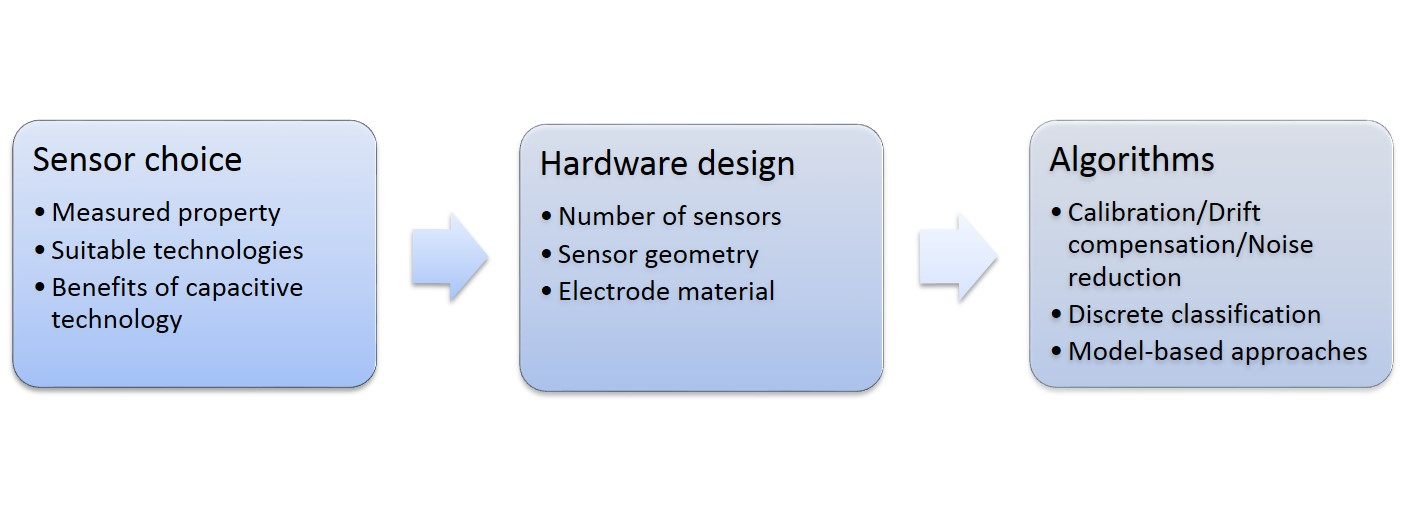
\includegraphics[width=0.8\textwidth]{images/guide_process}
\captionof{figure}{Basic system design process for capacitive proximity sensing systems and associated aspects in the single steps}
\label{fig:guide_process}
\end{minipage}

After discussing the limitations and benefits of capacitive proximity sensors, I am able to use the collected experiences and knowledge to give some general guidelines that can help parties interested in this sensing technology. These guidelines will support the design process from sensor choice, to choice of algorithms. The process is shown in Figure \ref{fig:guide_process}. This section is structured following the three design steps sensor choice, hardware design and algorithms and poses a set of questions in each subsection that are associated to the specific challenges. These questions will be answered with references to the design processes that have driven the creation of the different prototypes created in the scope of this work.
 
\subsection{Sensor choice}
The first step of this process is a decision if capacitive sensors technology is suitable for the given application. This part should be driven by three questions.

\textit{What do I need to measure in my application scenario?
}

Capacitive proximity sensors can measure the presence and properties of conductive, grounded objects. This includes the various application sce-narios shown in the previous sections. However, if the application requires measuring properties of unsupported objects that are non-conductive, a dif-ferent technology should be chosen.

\textit{What sensing technologies are supporting the required measurements?}

It may be the case that multiple technologies support the measurements required in this specific applications. Cameras often can provide similar recognition as capacitive sensors, e.g. in indoor localization applications. In this step all potential sensing technologies should be collected.

\textit{Are capacitive proximity sensors beneficial for my scenario?}

An evaluation of the different candidates is the final step and should lead to a decision about the most suitable sensing technologies. If the distance is too high for capacitive proximity sensors or enough processing power is available and lighting conditions are static, cameras might be more suitable. This should be driven by the different benefits and limitations of  the technologies.
If there is a decision in favor of capacitive sensors the next step is to design the specific electrode layout. Similar to technology selection we can use a few basic questions to get an idea of what layout to use.

\subsection{Hardware design}
\textit{How many sensors are required to get the measurement?}

The number of sensors required is depending on the area we want to cover, the specific object parameters that have to be determined and the desired resolution. The electrodes are inherently limited in size, as a single sensor can only charge and discharge to a specific maximum capacity. Therefore, if a large area has to be covered more electrodes and sensors are necessary. If we just want to measure the presence of a hand a single electrode may suffice. If orientation and position are interesting we need to combine measurements from various sensors. We used six electrodes for the MagicBox (\ref{ch:prot_magicbox}) as it is only tracking a single hand on a limited surface. Most prototypes (\ref{ch:prot_smartbed}, \ref{ch:prot_capchair}, \ref{ch:prot_armrest}) use eight sensors as this turned out to be a good compromise providing sufficient data that can be collected by a single sen-sor kit. CapTap (\ref{ch:prot_captap}) uses 24 sensors as we wanted a high resolution over a larger area and CapFloor \ref{ch:prot_capfloor} is scaled to room size and may use a high number of sensors.


\textit{What should be the size and geometry of the electrodes?}


This is closely related to the previous question. If the application is not restricting the available space, the electrode should be approximately of the same size as the object that is to be detected. This generates the highest difference in capacitance when the distance is changing. The Active Armrest (\ref{ch:prot_armrest}) uses six very small electrodes for finger tracking and two larger ones for detecting the arm presence. CapFloor (\ref{ch:prot_capfloor}) uses wire electrodes that are spread throughout the room to maximize coverage. The hand tracking devices (\ref{ch:prot_armrest}, \ref{ch:prot_magicbox}) are equipped with hand-sized electrodes and the body sensing devices (\ref{ch:prot_smartbed}, \ref{ch:prot_capchair}) use as much of the available space as possible.


\textit{What is the best electrode material to use?}


Copper is always a good first choice to create electrodes. If elasticity is necessary we can use copper foil and solid copper if that is of no concern. For transparent electrodes we will have to use one of the previously presented materials, such as ITO. If electrodes have to be integrated into cloth, conductive thread is a good candidate. Any conductive material will act as an electrode, thus the application and budget should be the primary driver of this decision. Active Armrest and CapTap (\ref{ch:prot_armrest}, \ref{ch:prot_captap}) are not con-strained and use solid copper electrodes. CapFloor (\ref{ch:prot_capfloor}) uses copper wires. MagicBox (\ref{ch:prot_magicbox}) integrates the sensors into a thin casing, thus we used aluminum foil. As we wanted the electrodes of the Smart Bed (\ref{ch:prot_smartbed}) to deform along with the slatted frame we used copper foil. The Capacitive Chair (\ref{ch:prot_capchair}) uses a number of solid copper electrodes but also includes a single conductive thread, as it could be integrated into the mesh structure of the back rest.


\textit{Does my application require any shielding?}


Shielding allows detecting only objects approaching from a certain direction. If the application requires this additional hardware, because it is anticipated that other objects might disturb the measurement, shielding should be used. The only prototype that uses shielding is the CapTap (\ref{ch:prot_captap}), as various electronic devices are integrated into the table and we wanted to minimize disturbance.

\subsection{Algorithms}
Finally, if the hardware is designed as desired the different variations of data processing have to be chosen and configured according to the application.

\textit{What pre-processing algorithms should be used?}

Using baseline calibration is beneficial in the vast majority of applications. Having a distinct starting point simplifies all further steps of high-level data processing, such as normalization and setting different thresholds. This step may only be omitted in very stable environments and if the system has sufficient a priori information to operate on raw data. Drift compensation should be handled in a similar fashion. The common methods are not computationally expensive and having a stable baseline over time allows the same algorithms to be applied in a more robust fashion. The method and configuration of noise reduction are strongly depending on the specific case. Some form of noise reduction might be required in most applications. Yet, according to the type of noise different methods can be used. If outliers are an issue a median filter is appropriate; if a smoother signal is desired an average filter can be used. 

\textit{What are suitable methods for high-level data processing?}

Regarding high-level data processing there are numerous variations of methods presented in this work. Data-driven machine learning algorithms are a good method, if we have a small set of potential outcomes, e.g. the different postures that could be recognized on a chair or couch. We partially use these methods in the Smart Bed (\ref{ch:prot_smartbed}) and exclusively regarding the posture classification of the Capacitive Chair (\ref{ch:prot_capchair}). If our application has many different potential outcomes, e.g. the thousands of potential locations in a hand tracking system, it is typically beneficial to use a model-driven approach, used in all other prototypes (\ref{ch:prot_capfloor}, \ref{ch:prot_armrest}, \ref{ch:prot_magicbox}, \ref{ch:prot_captap}). However, these models may be supported by data-driven algorithms, such as particle filters. One example is the Swiss-Cheese object tracker by Grosse-Puppendahl et al. \cite{grosse2013swiss}. The data processing examples shown in Section \ref{ch:prot_proc} give an idea of the decision rationale in various application domains.


